%\documentclass{standalone}
%
%% \usepackage{graphicx}
%\usepackage{epstopdf}
%\usepackage{tikz}
%\usetikzlibrary{shapes,arrows}
%% We need layers to draw the block diagram
\pgfdeclarelayer{background}
\pgfdeclarelayer{foreground}
\pgfsetlayers{background,main,foreground}

% Define a few styles and constants
\tikzstyle{individual}=[draw, fill=blue!20, text width=5em, 
    text centered] % , minimum height=1.5em]
\tikzstyle{individualtrans}=[draw, fill=green!20, text width=5em, 
    text centered] % , minimum height=1.5em]
\tikzstyle{ann} = [above, text width=5em]
\tikzstyle{dpmechs} = [individual, text width=6em, fill=red!20, 
    minimum height=12em, rounded corners]
\def\blockdist{2.3}
\def\rowdist{3.3}
\def\edgedist{2.5}
\def\arrowdist{1}

% \newcommand{\tname}{\textsc{TransformeR}}
% \newcommand{\dppsi}{\textsc{PSI}}

% \begin{document}
\begin{figure}
\begin{center}
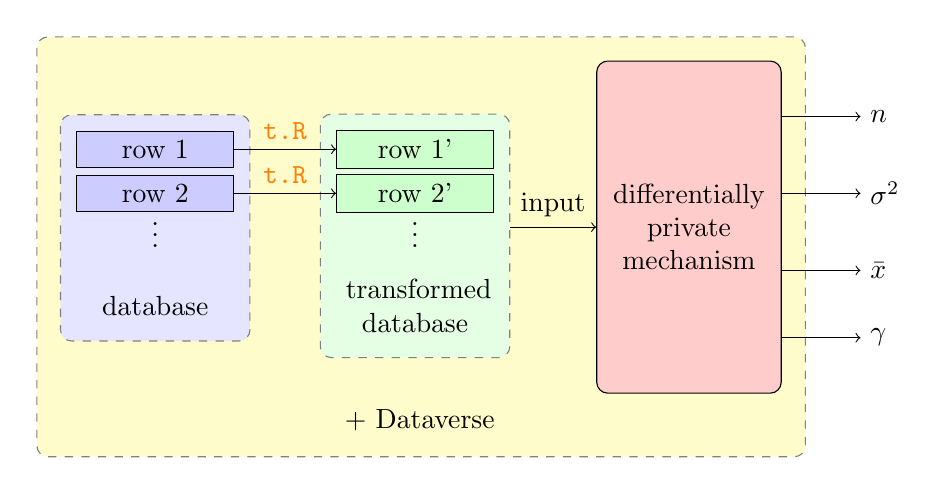
\begin{tikzpicture}
    \node (dpmech) [dpmechs] {differentially private mechanism};
    % Note the use of \path instead of \node at ... below. 
    \path (dpmech.140)+(-\blockdist,0) node (row1') [individualtrans] {row 1'};
    \path (dpmech.160)+(-\blockdist,0) node (row2') [individualtrans] {row 2'};
    \path (dpmech.180)+(-\blockdist,0) node (dots) {$\vdots$};

    \path (row1')+(-\rowdist,0) node (row1) [individual] {row 1};
    \path (row2')+(-\rowdist,0) node (row2) [individual] {row 2};
    \path (dots)+(-\rowdist,0) node (dots') {$\vdots$};
    
    % transformed database

    %\path [draw, ->] (row) -- node [above] {\texttt{t.R}} 
    %    (dpmech.west |- row) ;
    %% We could simply have written (row) .. (dpmech.140). However, it's
    %% best to avoid hard coding coordinates
    %\path [draw, ->] (row') -- node [above] {\texttt{t.R}}
    %    (dpmech.west |- row');
    %\node (database) [below of=row'] {database};
    % Unfortunately we cant use the convenient \path (fromnode) -- (tonode) 
    % syntax here. This is because TikZ draws the path from the node centers
    % and clip the path at the node boundaries. We want horizontal lines, but
    % the sensor and dpmech blocks aren't aligned horizontally. Instead we use
    % the line intersection syntax |- to calculate the correct coordinate
    %\path [draw, ->] (row1') -- node [above] {\texttt{t.R}} 
    %    (dpmech.west |- row1') ;
    %% We could simply have written (row) .. (dpmech.140). However, it's
    %% best to avoid hard coding coordinates
    %\path [draw, ->] (dpmech |- row2'.east) -- node [above] {\texttt{t.R}}
    %    (dpmech);
    \node (database') [text width=5em, align=center, below of=dots] {transformed database};

    \path [draw, ->] (row1) -- node [above] {\color{orange} \texttt{t.R}}
        (row1') ;
    % We could simply have written (row) .. (dpmech.140). However, it's
    % best to avoid hard coding coordinates
    \path [draw, ->] (row2) -- node [above] {\color{orange} \texttt{t.R}}
        (row2');
    \node (database) [below of=dots'] {database};

    % \path (dpmech.south west)+(-0.6,-0.4) node (PSI) {\dppsi{} + Dataverse};
    \path (database'.south)+(0, -1.0) node (PSI) {\dppsi{} + Dataverse};
    \draw [->] (dpmech.50) -- node {} + (\arrowdist,0) 
        node[right] {$n$};
    %\draw [->] (dpmech.50) -- node [ann] {count} + 
    %    node[right] {$n$};
    \draw [->] (dpmech.20) -- node {} + (\arrowdist,0) 
        node[right] { $\sigma^2$};
    \draw [->] (dpmech.-25) -- node {} + (\arrowdist,0) 
        node[right] { $\bar{x}$};
    \draw [->] (dpmech.-50) -- node {} + (\arrowdist,0) 
        node[right] {$\gamma$};

    \draw [->] (row1'.east |- dpmech)+(0.2,0) -- node [above] {input} (dpmech);
    
    % Now it's time to draw the colored database and INS rectangles.
    % To draw them behind the blocks we use pgf layers. This way we  
    % can use the above block coordinates to place the backgrounds   
    \begin{pgfonlayer}{background}
        % Compute a few helper coordinates
        \path (row1.west |- dpmech.north)+(-0.5,0.3) node (a) {};
        \path (PSI.south -| dpmech.east)+(+0.3,-0.2) node (b) {};
        \path[fill=yellow!20,rounded corners, draw=black!50, dashed]
            (a) rectangle (b);

        \path (row1.north west)+(-0.2,0.2) node (a) {};
        \path (database.south -| row1.east)+(+0.2,-0.2) node (b) {};
        \path[fill=blue!10,rounded corners, draw=black!50, dashed]
            (a) rectangle (b);

        \path (row1'.north west)+(-0.2,0.2) node (a) {};
        \path (database'.south -| row1'.east)+(+0.2,-0.2) node (b) {};
        \path (database'.north -| row1'.east)+(-0.2,+0.2) node (c) {};
        \path [fill=green!10,rounded corners, draw=black!50, dashed]
            (a) rectangle (b) node (d) {};
        %\draw [->] (d.east |- dpmech) -- (dpmech);

    \end{pgfonlayer}
\end{tikzpicture}
\end{center}
\caption{Integration of \tname{} in \dppsi{}. The analyst defines 
  variable transformation in file {\color{orange} \texttt{t.R}}}
\label{fig:psiintegration}
\end{figure}
% \end{document}
